%Dies ist das Hauptdokument!

%Dieses Hauptdokument bearbeitet nur der Redakteur.
%Die einzelnen Autoren m�ssen sich �berhaupt nicht um den gew�hnungsbed�rftigen
%Vorspann k�mmern sondern nur ASCII-Text schreiben und ihren Text mit
%einigen wenigen Befehlen logisch gliedern. Um Schriftarten, -gr��en, Kopf- und
%Fu�zeilen k�mmert sich ausschlie�lich die Redaktion.

\documentclass[titlepage,a4paper,twoside,11pt]{report}

% \input{parameter.tex}

%
% Spezielle Header/Footer verwenden
%

\usepackage{fancyhdr}
% \usepackage{ngerman} % neue deutsche Rechtschreibung
\usepackage[T1]{fontenc}
\usepackage[latin1]{inputenc}
\usepackage[pdftex]{graphics}
\usepackage[pdftex]{rotating}
%\usepackage{europs} %EURO-Zeichen mit \EUR\ oder \EURofc\
\sloppy
\usepackage{graphicx}
\usepackage{epsfig}
\usepackage{latexsym}
\usepackage{multicol}
\usepackage{longtable}
\usepackage{color}
\usepackage{makeidx}
\makeindex
%\usepackage{dropping} % Initialen verwenden
\DeclareGraphicsRule{.tif}{.bmp}{.jpg}{}
%\DeclareGraphicsExtensions{.jpg,.pdf,.mps,.png,.eps}

%Includefiles festlegen
%\includeonly{2302linpro}
%------------------------
% einige Variablen f�r Seitenumbr�che anpassen
%

\renewcommand{\floatpagefraction}{.9}% vorher: .5
\renewcommand{\textfraction}{.02} % vorher: .2
\renewcommand{\topfraction}{.8}     % vorher: .7
\renewcommand{\bottomfraction}{.5}  % vorher: .3

%
% Neue Befehle von Mattias f�r eigene Absatzformate
%

\newcommand{\zpgsection}[1]{\section*{\raggedright \huge \sffamily {#1}}
\addcontentsline{toc}{section}{#1} \def\pagetitle{#1}}
\newcommand{\zpgsubsection}[1]{\subsection*{\mdseries \textbf {#1}}
\addcontentsline{toc}{subsection}{#1}}
\newcommand{\zpgsubsubsection}[1]{\subsubsection*{\mdseries \textbf {#1}}
\addcontentsline{toc}{subsubsection}{#1}}
\newcommand{\zpgleit}[1]{\noindent \emph{#1}}

% ...dann geht es mit \zpgsection{Artikelueberschrift} und
% \zpgsubsection{Unterueberschrift}!

%%%%%%%%%%%%%%%%%%%%%%%%%%%%%%%%%%%%%%%%%%%%%%%%%%%%%%%%%%%%
% Aenderungen von Mattias
%%%%%%%%%%%%%%%%%%%%%%%%%%%%%%%%%%%%%%%%%%%%%%%%%%%%%%%%%%%%
% Echten Euro nur verwenden falls vorhanden

\IfFileExists{europs.sty}{\usepackage{europs}\newcommand\euro{\EUR}}
			{\newcommand\euro{{\sffamily C%
    			\makebox[0pt][l]{\kern-.70em\mbox{--}}%
    			\makebox[0pt][l]{\kern-.68em\raisebox{.25ex}{--}}}}}
% andernfalls: erzeugt provisorisches EURO-Symbol

\usepackage{colortbl}
\usepackage{pifont}
\newcommand{\Achtung}{\subsubsection*{\textcolor{red}{Achtung:}}}
\newcommand{\Warning}{\subsubsection*{\textcolor{red}{Warning:}}}
\newcommand{\Beispiele}{\subsubsection*{Beispiele:}}
%\newcommand{\Parameter}{\subsubsection*{Parameter:}}
\definecolor{darkblue}{rgb}{0.15,0.15,0.57}

%%%%%%%%%%%%%%%%%%%%%%%%%%%%%%%%%%%%%%%%%%%%%%%%%%%%%%%%%%%%%

%\setlength{\paperwidth}{29.7cm}
%\setlength{\paperheight}{21cm}
%\setlength{\textwidth}{27cm}
%\setlength{\textheight}{18cm}

%
% Bedruckten Bereich vergr��ern
%

\setlength{\textheight}{24cm} \setlength{\textwidth}{16cm}
\setlength{\oddsidemargin}{0.0cm} \setlength{\topmargin}{0cm}
\setlength{\evensidemargin}{0.0cm} \setlength{\columnsep}{18pt}
\setcounter{topnumber}{8} % vorher: 2
\setcounter{bottomnumber}{5} % vorher: 1
\setcounter{totalnumber}{10} % vorher: 3


%%%%%%%%%%%%%%%%%%%%%%%%%%%%%%%%%%%%%%%%%%%%%%%%%%%%%%%%%
%�nderungen von Andrea:
%%%%%%%%%%%%%%%%%%%%%%%%%%%%%%%%%%%%%%%%%%%%%%%%%%%%%%%%%
%Der folgende Befehl definiert die Verwendung von \url ...
\IfFileExists{url.sty}{\usepackage{url}}
                      {\newcommand{\url}{\texttt}}
%kein Einr�cken, wenn ein neuer Absatz beginnt:
%\parindent0cm
%%%%%%%%%%%%%%%%%%%%%%%%%%%%%%%%%%%%%%%%%%%%%%%%%%%%%%%%%
%
% Anpassungen f�r Seitenkopf
%


%\def\pagetitle{}

    \pagestyle{fancy}
        \fancyhead[LE,RO]{\thepage}
        \fancyhead[RE]{\textsf {LessLinux Handbook}}
        \fancyhead[LO]{\textsf {\pagetitle}}

     \fancyfoot[C]{}
%
% Ende - Anpassungen f�r Seitenkopf
%


% \usepackage{ae}       % zur Suche nach Worten mit Umlaut
                           % noetig

%
% PDF-Optionen:
%

%%%% Zur PDF-Erzeugung (Hyperlinks) ben�tigte Optionen
%%%% Details siehe Dokumentation von hyperref, bei jeder
%%%% teTeX-Distribution >= 1.0.6 dabei.

%%%% Bitte ganz am Schlu� unterbringen,
%%%% da viele Befehle neu definiert werden

\usepackage{ae}       % zur Suche nach Worten mit Umlaut
                      % noetig
\usepackage{palatino}
%\usepackage{times}   % Type-1-Schriften
                      % (nicht immer notwendig)
\usepackage[
   a4paper,      % A4
   pdftex,        % Erzeugung durch dvips
   pdftitle={LessLinux Handbook},
       pdfauthor={Mattias Schlenker},
   bookmarks=true,
       bookmarksopen=true,     % Bookmarks anzeigen...
       bookmarksnumbered=true, % ...und numerieren
   colorlinks,   % Farbige Links
	linkcolor=darkblue,
     urlcolor=darkblue]{hyperref}


\newcommand{\Parameter}[1]{\subsubsection*{\hypertarget{#1}{Parameter}}}

%\usepackage[dvips]{thumbpdf}
%Beginn des Inhalts der Zeitschrift
%%%%%%%%%%%%%%%%%%%%%%%%%%%%%%%%%%
\begin{document}

\title {}

\author{Mattias Schlenker}
\date  {\today}
%\maketitle
\def\pagetitle{}
MENU TITLE LessLinux BigFatFull 0.1


\def\pagetitle{Inhaltsverzeichnis}
\tableofcontents
\newpage
\def\pagetitle{lesslinux.com Documentation}
%Angabe der Schriftart
%\sffamily                 %serifenlos
\normalfont                %normal
%%%%%%%%%%%%%%%%%%%%%%%%%%%%%%%%%%%%%%%%%%%%%%%%%%%%%%%%%%%%%%%%%%%%%%%%%%%%%%%%%%%%%%%%%%%%%%%%
%Eingef�gte Artikel

\begin{abstract}
LessLinux is a free Linux system designed to be light and easily modifiable. It is based on \href{http://www.linuxfromscratch.org}{Linux from Scratch}  and was started by Mattias Schlenker in 2009. Since then it has been used as a base for dozens of security and rescue systems published by computer magazines all over the world. It's simple architecture makes it easy to build LessLinux based systems for use as thinclient, software deployment or the demonstration of software. This book covers the possibilities of LessLinux and tells you how small changes can make LessLinux the lever you need to move your world.  
\end{abstract}

\chapter{About LessLinux and this handbook}
\chapter{LessLinux for users}
\chapter{LessLinux for admins}

This chapter covers using LessLinux for typical administrative tasks in heterogenous networks. Topics will be remote accessing a macine running LessLinux, using LessLinux as a simple yet flexible thinclient and booting LessLinux via the network. It will further cover modifying lesslinux with payloads: An easy way to add scripts (like for backing up and restoring), thus using LessLinux as a platform for your own netbootable toolbox  - without having to touch LessLinux containers.



\hypertarget{remote}{} 
\section{Remote access}

Since one of the main target groups for LessLinux are network admins, easy remote access to running LessLinux instances was one of the goals during development. Currently access via \index{SSH} SSH and \index{VNC} VNC is supported, both together result in encrypted VNC. Reverse VNC allows for easy remote support on machines that are behind NAT routers and firewalls. RDP access is work in progress. 

\hypertarget{ssh}{} 
\subsection{SSH}

LessLinux is usually shipped with the OpenSSH secure shell server. However this is disabled in most builds by adding it to the \texttt{skipservices=|servic1|service2|} boot command line. To start the OpenSSH server, remove \texttt{ssh} from \texttt{skipservices}.

\Warning{
Placing the hash for the root password in the boot command line, transferring it over a hostile network or netbooting with SSH machine keys (or root's private SSH keys) make eavesdropping easy. Use those options just in networks that are considered safe. Also consider locking down the local consoles when LessLinux is netbooted in order to do adminstrative tasks via SSH to prevent local users from manipulating the machine.
}

\subsubsection{Login with password}

To login with password use the possibility to add files to the initramfs by adding \texttt{/etc/lesslinux/root.hash} that contains the MD5 hash of the root password. You can generate this hash with the command

\begin{verbatim}
openssh passwd -1 
\end{verbatim}

You might also specify the base64 encoded MD5 hash of the root password via boot command line. Since the \texttt{=} character which is used for indicating padding in base64 is not valid, you will have to pad the hash with one or more spaces (usually one) until the base64 string does not end on \texttt{=}. Those spaces are removed after decoding:

\begin{verbatim}
hash=` openssl passwd -1 `
echo "$hash " | base64 
\end{verbatim}

The result must look like:

\begin{verbatim}
JDEkTktlL3NSRHIkd1owLzJ5UjJDTVdlMnZPY0NaSGRuMSAK
\end{verbatim}

The resulting parameter for the boot command line:

\begin{verbatim}
roothash=JDEkTktlL3NSRHIkd1owLzJ5UjJDTVdlMnZPY0NaSGRuMSAK
\end{verbatim} 

\subsubsection{Public key login}

Use the possibility to add files to the initramfs by preparing a CPIO archive that contains all the host keys placed in \texttt{/etc/openssh} as well as the needed \texttt{/root/.ssh/authorized\_keys}. Make sure permissions fit and add this CPIO archive as the last file to the bootloader or concatenate it to the initramfs if you use a bootloader that allows just one initramfs. If permissions are correct and the OpenSSH daemon is started you can connect with public key login afterwards.

\subsection{VNC}

Virtual Network Computing or \emph{VNC} is a simple, easy to implement protocol used to gain access to remote computers. It is the basis for Apple's remote administration tool. Clients are available for nearly every operating system as well as for smartphones and as Java applet. In LessLinux VNC can be used to mirror a local X server - which can be either a graphical console or an invisible virtual frame buffer.

\Warning{The VNC protocol does not use encryption! This means all keyboard input and all screen output can easily be eavesdropped. Combine VNC with an SSH tunnel if you need some minimum security.}

\subsubsection{VNC for incoming connections}

The easiest way to access a running LessLinux system is mirroring the local Xserver. Specify

\begin{verbatim}
x11vnc=|remote|
\end{verbatim}

to enable VNC access without password. You might specify a clear text password as second argument:

\begin{verbatim}
x11vnc=|remote|password|
\end{verbatim}

VNC uses port 5900 as default. The current IP address is usually shown on the first console (\texttt{Ctrl+Alt+F1}). 

\subsubsection{Reverse VNC}

If a host that booted LessLinux is running behind a firewall or NAT router, incoming connections might not be possible. With reverse VNC the LessLinux host tries to establish an outgoing connection to the IP address or hostname specified as target (on port 5500):

\begin{verbatim}
x11vnc=|reverse|target|
\end{verbatim}

On a Linux target machine you usually run 

\begin{verbatim}
vncviewer -listen
\end{verbatim}

or use the graphical application Remmina to work with reverse VNC connections.

\subsubsection{Headless access}
 
Specify \texttt{x11vnc=...} as mentioned above to enable VNC access. To run headless access instead of the local X server you have to disable it and replace it by Xvfb - the virtual frame buffer X server, which is done with the additional parameter 

\begin{verbatim}
xvfb=1280x800x32
\end{verbatim}
 
The \texttt{1280x800x32} tells Xvfb to start with an 1280x800 resolution and 32 bit color depth. All values that make sense (they should resemble real world resolutions) are allowed.

\subsubsection{Tunnel VNC over SSH}

The security implecations of VNC are described earlier in this chapter. If you want to use VNC in hostile environments, enable  \hyperlink{ssh}{SSH access}. Then bind the listening port for VNC to localhost only by specifying:

\begin{verbatim}
x11vnc=|local|
\end{verbatim}

On the machine that is used to access the LessLinux with running VNC you then have to run SSH with port forwarding, on unix like operating systems:

\begin{verbatim}
ssh -L 5900:localhost:5900 lesslinux-host
\end{verbatim}

On the machine connecting via SSH, VNC's port 5900 is now available at \texttt{localhost}, point your VNC viewer to \texttt{localhost} or \texttt{127.0.0.1}. Depending on the viewer it may be necessary to specify the priority of encodings (if you are using \texttt{vncviewer} from TightVNC, see the man page regarding \texttt{-encodings}.

\subsection{RDP}

Remote access via Microsofts Remote Desktop Protocol \index{RDP} based on \texttt{xrdp} is in experimental state. Specify 

\begin{verbatim}
xrdp=1
\end{verbatim}

to enable the VNC-to-RDP gateway. This requires a running VNC server, at least listening on the local loopback interface. Of course you can enable RDP with an VNC server that mirrors the local display or headless. We suggest using

\begin{verbatim}
x11vnc=|local|secret| xvfb=1280x800x16 xrdp=1
\end{verbatim}

to enable a headless VNC server that listens on 127.0.0.1, color depth fset to 16 bit. The password ,,secret'' will then be prompted upon RDP login. All traffic is encrypted which minimizes the risk of sniffing.

\begin{figure}[htbp]
\center{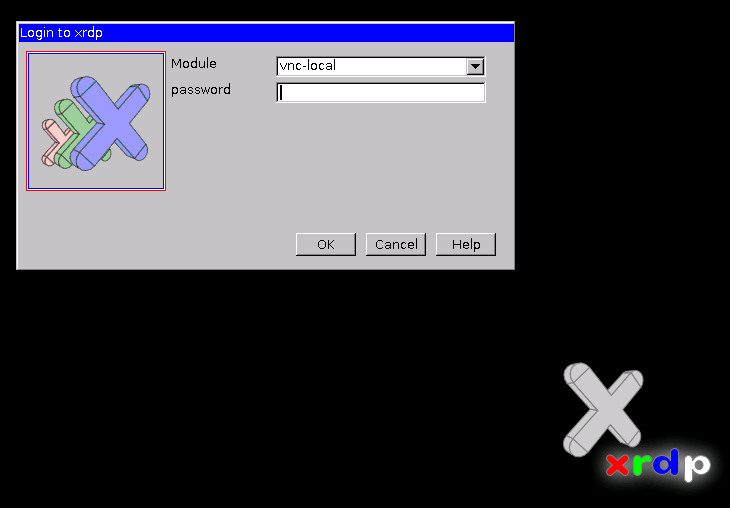
\includegraphics[width=8cm]{admin/xrdp.png}}
\caption{\label{fig:xrdp} Xrdp provides a simple VNC-to-RDP gateway, this comes handy if you want to access a machine running LessLinux from a Windows machine.}
\end{figure}

\subsection{Xpra}

,,X persistent remote applications'' is a relatively unknown, yet very efficient way of saemlessly exporting X11 applications to another computer. See \href{https://www.xpra.org}{www.xpra.org} for details.  The connection between machines is usually done with a SSH tunnel. If the connection is lost, all applications and usually even their positions are restored upon re-connect. Xpra needs a running SSH server, so make sure to enable it and set a password or provide a key before enabling Xpra. Enable Xpra with

\begin{verbatim}
xpra=1
\end{verbatim}

Then connect on another computer with Xpra installed with the command:

\begin{verbatim}
xpra attach ssh:root@12.34.56.78:100 
\end{verbatim}

After providing the password you will get a single terminal window from which you can start any X11 application. To change the default app that is started, provide the full path when enabling Xpra:

\begin{verbatim}
xpra=/path/to/program
\end{verbatim}







\section{Netbooting LessLinux}

Netbooting LessLinux is a convenient way of providing a rescue system to medium scale networks or converting existing machines to thin clients. To maximize the possiblities you might want to combine netboot with \hyperlink{remote}{remote access} or \hyperlink{thinclient}{LessLinux as thin client}.  

This chapter will not describe how to completely setup a netboot environment. Please view the respective documentation of your preferred DHCP server and TFTP daemon to see how to get kernel and initramfs delivered to your PXE capable clients. For the system's boot command line boot LessLinux from CD and then run

\begin{verbatim}
cat /proc/cmdline
\end{verbatim}

to retrieve a command line that can be used as a basis for the the following examples. Make sure that \texttt{earlynet} is not included in the list of services to skip, since this brings up network interfaces before the system image is found. To speed up boot you might add \texttt{dhcpcd} and \texttt{wicd} to the list of services to skip.

\Warning{Builds after 20130717 use the variable \texttt{defermods} to mount a tmpfs over all module directories specified here. To speed up start and make firmware loading more reliable this delegates loading of ethernet drivers to after the containers are mounted. So if you want to still be able to netboot, set

\begin{verbatim}
defermods=|drivers/net/wireless|drivers/gpu/drm|sound|
\end{verbatim}

at the boot command line.}

\subsection{CIFS or NFS boot}

With the command line

\begin{verbatim}
nfs=12.34.56.78:/path/to/share
\end{verbatim}

respectively

\begin{verbatim}
cifs=//12.34.56.78/share
\end{verbatim}

the specified share will be mounted during boot. The share will then be recursively searched for an ISO image that matches the LessLinux build running. This ISO will then be loopback mounted. Please note that when using  \texttt{cifs} the share must be mountable as User \texttt{guest} with an empty password. 

Depending on speed and reliability of your network and RAM of your clients you might want to use \texttt{toram=1} to force loading the system completely to memory upon boot. This might cost about one minute during startup, but will accelerate the start of programs considerably in congested networks.

This boot method is defined in \texttt{/etc/rc.d/0107-nfssys.sh}.

\subsection{HTTP, FTP or TFTP boot}

Use the command line parameter 

\begin{verbatim}
wgetiso=http://12.34.56.78/path/to/image.iso
\end{verbatim}

to use BusyBox' \texttt{wget} to download LessLinux' ISO image. The complete ISO image will be saved in memory, so this option requires sufficient RAM. Using \texttt{tftp} as alternative protocol allows netbooting without having to setup another daemon on your server. However \texttt{tftp} is far less reliable, so this should be just used as an option if no other protocol is available. 

This boot method is defined in \texttt{/etc/rc.d/0108-wgetsys.sh}.

\Warning{Always make sure the parameter \texttt{toram=0} prevents that LessLinux will be copied to RAM again. Activated \texttt{toram} would double the amount of RAM used for the system!}






%%%%%% 

\section{LessLinux as thinclient}

Since autumn 2012 LessLinux includes programs and scripts to run as a thinclient with minimal overhead. This targets primarily environments where LessLinux is booted via the network and converted to a thinclient OS with just a few boot parameters. For now the functionality to comfortably access \index{RDP} RDP logins is implemented, audio redirection works good if optional parameters are specified (chooser only). Access to printers, local USB drives and other local USB devices is work in progress.

\subsection{Booting to Remmina}

\begin{figure}[htbp]
\center{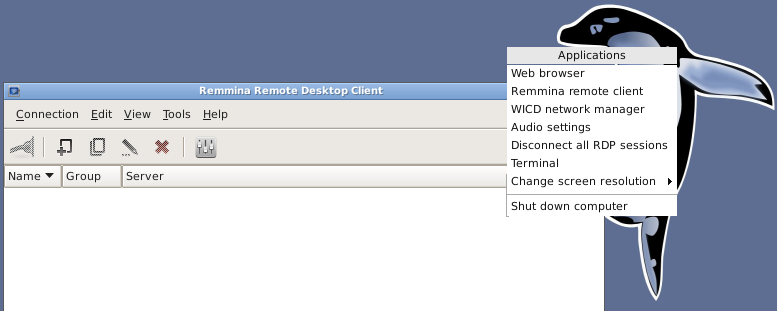
\includegraphics[width=12cm]{admin/remmina.png}}
\caption{\label{fig:remmina} Just specifying \texttt{xinitrc=/etc/lesslinux/xinitrc\_remote} will open Remmina on an otherwise empty desktop. Right click on the desktop background to get a menu with some useful programs (also available when booting to chooser or RDP login mask).}
\end{figure}

If you just pass the parameters 

\begin{verbatim}
xinitrc=/etc/lesslinux/xinitrc_remote
\end{verbatim} 

you will end up in an empty desktop with a \index{Remmina} Remmina window open. Remmina allows for access to RDP, VNC, reverse VNC and SSH servers. Since all settings are lost upon reboot, this option is primarily interestinng for admins who want to be able to remotely login to servers from any machine in the network that boots via PXE.

With the \texttt{xinitrc\_remote}
the default window manager is OpenBox. Right click on the desktop to get a simple menu from where you can start Firefox, a terminal window or the mixer (for remote audio). 

\subsection{Booting to an RDP login mask}

\begin{figure}[htbp]
\center{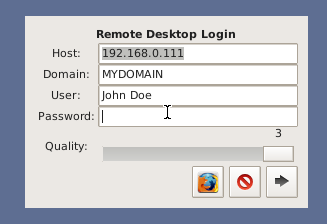
\includegraphics[width=8cm]{admin/rdpmask.png}}
\caption{\label{fig:rdpmask} The RDP login mask is configured via boot command line and does not need a separate configuration file.}
\end{figure}

The easiest way is booting to a simple login mask: To enable thinclient mode specify

\begin{verbatim}
xinitrc=/etc/lesslinux/xinitrc_remote
\end{verbatim} 
 
and additionally to enter the RDP login mask

\begin{verbatim}
rdesktop=|12.34.56.78|username|domain|2|
\end{verbatim} 

Those parameters are IP address of the RDP server, user name and domain name (optional). The user name might be encoded as in HTTP URIs: \texttt{Kemal\%20Atat\%C3\%BCrk} is unescaped to \texttt{Kemal Atat�rk} - however due to character set limitiations you should try to avoid umlauts in user names. The optional integer specifies the quality of the connection: 0 is low quality, but fast, 3 is highest quality, but slower. Use 0 for very slow connections (modem, 3G), 1 in broadband connections (or 3.5G, 4G), 2 (default) in typically congested ethernets and 3 for very fast ethernets with low congestion. Those numerical values map to the following parameters upon execution of \texttt{xfreerdp}

\begin{itemize}
\item \textbf{0} \texttt{-x m -a 16}  - 16 bit color depth, modem experience
\item \textbf{1} \texttt{-x b -a 16}  - 16 bit color depth, broadband experience
\item \textbf{2} \texttt{-x l -a  32} - 32 bit color depth, LAN experience
\item \textbf{3} \texttt{-x 180 -a  32} - 32 bit color depth, LAN experience plus font smoothing and Desktop Composition
\end{itemize}

RDP Sessions start in full screen. You might toggle full screen with \texttt{Ctrl+Alt+Enter}, e.g. to access the local OpenBox menu or start a local Firefox instance.

\subsection{Booting to a chooser}

\begin{figure}[htbp]
\center{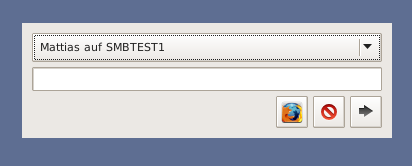
\includegraphics[width=8cm]{admin/chooser.png}}
\caption{\label{fig:chooser} The chooser is configured by an XML file that is loaded from the boot medium or via the network.}
\end{figure}

More comfort and more flexibility is provided by the optional chooser. To use it, you have to prepare an XML file with one block per entry. This XML file has to be accessible via FTP, HTTP or TFTP. Currently only RDP connections are available via chooser, \index{VNC} VNC, Nomachine NX, XDMCP and Citrix \index{ICA} ICA will follow eventually. Add the parameters 

\begin{verbatim}
xinitrc=/etc/lesslinux/xinitrc_remote
\end{verbatim} 
 
and

\begin{verbatim}
chooser=tftp://server/path/chooser.xml 
\end{verbatim} 

to boot into chooser mode. If you are booting from a USB drive, you can put the \texttt{chooser.xml} on the boot partition (usually the second partition on the thumb drive) and specify 

\begin{verbatim}
chooser=file:///lesslinux/boot/chooser.xml 
\end{verbatim}

Alternatively when remastering a CD with \texttt{chooser.xml} in the root directory of the ISO 9660 file system, specify 

\begin{verbatim}
chooser=file:///lesslinux/cdrom/chooser.xml 
\end{verbatim}

In both cases make sure to specify \texttt{toram=0} to prevent LessLinux from unmounting \texttt{/lesslinux/boot} or \texttt{/lesslinux/cdrom} before the chooser.xml there can be used.

A sample XML file \texttt{chooser.xml} could look like:

\begin{verbatim}
<chooser>
  <connect nicename="John Doe" host="192.168.0.23" 
           proto="rdp" user="john" domain="MYDOMAIN">
    <default inet="192.168.0.17" />
    <default ether="00:24:8c:6b:5d:e4" />
    <param>-x l -a 32</param>
  </connect>
  <connect nicename="Jane Doe" host="192.168.0.23" 
           proto="rdp" user="jane" domain="MYDOMAIN">
    <default inet="192.168.0.18" />
    <param>-x 180 -a 32</param>
    <param>--plugin rdpsnd --data tsmf:audio:alsa:plughw:0,0 --</param>
  </connect>
  <connect nicename="Alice X" host="192.168.0.24" 
           proto="rdp" user="alice" domain="OTHERDOMAIN">
    <default inet="192.168.0.19" />
    <param>-x l -a 32</param>
  </connect>
  <connect nicename="Admininstrator on Server 1" host="192.168.0.23" 
           proto="rdp" user="Administrator" />
  <connect nicename="Admininstrator on Server 2" 
           host="192.168.0.24" proto="rdp" user="Administrator" />
</chooser>
\end{verbatim}

The first to entries specifiy connections to the RDP server \texttt{192.168.0.23}, with the domain \texttt{MYDOMAIN}. The parameters specify LAN experience for John Doe and remote audio as well as font smoothing and compositing for Jane Doe. The \texttt{default} tag specifies on which client machines an entry is selected as default. On the client machines with local MAC adress  \texttt{00:24:8c:6b:5d:e4} or local IP \texttt{192.168.0.17} John Doe will be shown as default, on \texttt{192.168.0.18} Jane Doe will be shown as default. Feel free to play with parameters for \texttt{xfreerdp} to get the best performance according to your network's latency, bandwidth and congestion.

\subsection{Using XDMCP}

The X Display Manager Control Protocol \index{XDMCP} that is used in several unix only environments is work in progress and not yet reflected in any cheatcodes. It will become available soon with the sole limitation that the keymap of the initially started X server will be US english. Depending on your Display Manager some special character in passwords won't be at the used keys. As soon as you are logged in most desktop environments take care for setting the user's keyboard layout.

\subsection{Local printers}

\begin{figure}[htbp]
\center{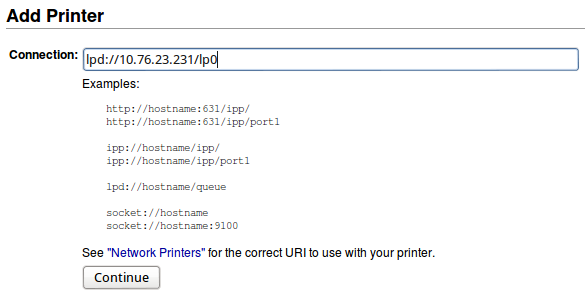
\includegraphics[width=12cm]{admin/printer.png}}
\caption{\label{fig:printers} Local USB printers can easily be shared: This screenshot shows adding USB printer \texttt{/dev/usb/lp0} on LessLinux host 10.76.23.231 to a CUPS server that centralizes spooling.}
\end{figure}

Minimal support for local printers is now provided with BusyBox' LPD. This is considered experimental, it might work or not, and parameters will change in the future without further notice. Specify 

\begin{verbatim}
printers=|lp0|lp1|
\end{verbatim} 

to enable printing to the USB printers available at \texttt{/dev/usb/lp0} and \texttt{/dev/usb/lp1}. This will start a line printer daemon with queues having the same names as the printers \texttt{lp0} and \texttt{lp1}. Since no filtering is done, the clients printing have to send raw output in a format the printer understands.




\chapter{LessLinux for builders and contributors}

The build system used by LessLinux is closely based on Linux from scratch. Building is done in three stages. The first stage is used to cross compile a toolchain that resides under \texttt{/tools}. In the second stage we use this toolchain to build all LessLinux packages in a chroot environment. Stage three is the assembly of the final boot image by taking the required files from the second stage. Although the fiirst stage involves cross compiling, the rest of the build process has to be done on the target architecture -- which currently only is i686. This means you should be able to build on any recent 32 Bit linux. Our preferred build environment  are the ,,FULL'' ISO images of LessLinux Search and Rescue that are self containing, you should also get good results using the latest Ubuntu LTS version. The next sections in this chapter tell you how to build using the LessLinux ,,FULL'' live ISO.

The examples in this chapter use the ,,FULL'' ISO image with it's defaults. We assume that you can leave the defaults, although some might seem odd: The build partition is mounted at \texttt{/mnt/archiv} (german diction without trailing ,e') and the unprivileged user for stage01  is called ,,mattias''. You can adjust these values in the settings contained in the \texttt{config} directory, but we do not recommend so for the first steps.

\section{Preparation}

\subsection{Prepare a drive}

We strongly recommend building LessLinux on a SSD with at least 40 Gigabyte you can dedicate to LessLinux - random access to small files is the most costly operation when building LessLinux. However, for the fist steps a notebook and a 32 Gigabyte USB thumb drive might do -- albeit much slower. Building on a virtual machine also works very good as long as you try to avoid fragmented hard disk images on rotational drives.

Prepare two partitions for the LessLinux build. They do not necessarily have to reside on the same hard disk, nor is a special partition scheme necessary - GPT and MBR will both work. Recommended size for the swap partition is 4 Gigabyte, the build partition itself should be between 20 and 60 Gigabytes. Larger sizes do not make any sense. Format them using a label that will be used to identify them when mounting:

\begin{verbatim}mkswap -L LessLinux_swap /dev/sdb1
mkfs.btrfs -L LessLinux_build /dev/sdb2
\end{verbatim} 

After preparing the disk(s), either reboot LessLinux with the ,,FULL'' ISO or run the following command:

\begin{verbatim}/usr/share/lesslinux/auxiliary-scripts/prepare-lesslinux-build.sh\end{verbatim}

This command will be run everytime upon boot in the ,,FULL'' ISO, so with the right labels you do not have to care about mounting anymore.

\subsection{Create some directories}

Some directories are not automatically created during the build process. This is intentional since you might want to share the sources directory between several machines building LessLinux. Create them manually as soon as \texttt{/mnt/archiv/LessLinux} is available: 

\begin{verbatim}mkdir -p /mnt/archiv/LessLinux/src
mkdir -p /mnt/archiv/LessLinux/llbuild
mkdir -p /mnt/archiv/LessLinux/llbuilder\end{verbatim}

\subsection{Download the ,,sources''}

The ,,sources'' are really just build definitions - shell script fragments embedded in XML files - and download locations. Currently those download locations are also backed up at \texttt{http://distfiles.lesslinux.org/}. This location is provided for build convenience and satisfaction of the GPL/LGPL only. If you distribute modified builds of LessLinux you have to provide your own sets of build definitions and sources (either downloads or physically), so do not count on me.

Build definitions are currently just available as tarballs that unpack in \texttt{/mnt/archiv/LessLinux/llbuilder}, subversion access might or might not follow. Just take the build definitions that seem to fit best to your planned LessLinux derivative. If unsure, take the latest source used to build LessLinux Search and Rescue:

\begin{verbatim}wget -O /tmp/llsrc.tar.xz \
http://download.lesslinux.org/src/\
lesslinux-search-and-rescue-uluru-YYYYMMDD-HHMMSS-buildscripts.tar.xz\end{verbatim}

Unpack the build scripts in the newly created directory llbuilder:

\begin{verbatim}cd /mnt/archiv/LessLinux/llbuilder
tar xvJf /tmp/llsrc.tar.xz\end{verbatim}








\section{Build the first stage}

 

\printindex 

%%%%%%%%%%%%%%%%%%%%%%%%%%%%%%%%%%%%%%%%%%%%%%%%%%%%%%%%%%%%%%%%%%%%%%%%%%%%%%%%%%%%%%%%%%%%%%%%%%

\end{document}
